\documentclass[14pt]{article}

\usepackage[utf8x]{inputenc}
\usepackage[russian]{babel}
\usepackage{graphicx}
\graphicspath{{images/}}
\DeclareGraphicsExtensions{.pdf,.png,.jpg}

\usepackage{amsmath}
\usepackage{pgfplots}

\usepackage{geometry} % Меняем поля страницы
\geometry{left=2cm}% левое поле
\geometry{right=1.5cm}% правое поле
\geometry{top=2cm}% верхнее поле
\geometry{bottom=2cm}% нижнее поле

\renewcommand{\theenumi}{\arabic{enumi}}
\renewcommand{\labelenumi}{\arabic{enumi}}
\renewcommand{\theenumii}{.\arabic{enumii}}
\renewcommand{\labelenumii}{\arabic{enumi}.\arabic{enumii}.}
\renewcommand{\theenumiii}{.\arabic{enumiii}}
\renewcommand{\labelenumiii}{\arabic{enumi}.\arabic{enumii}.\arabic{enumiii}.}

\begin{document}
\begin{titlepage}
	\begin{center}
		\fontsize{18pt}{20pt}\selectfont
		\textbf{Работа 4.3.2}	
	
		\vspace{5cm}
		\fontsize{24pt}{25pt}\selectfont
		Дифракция света на ультразвуковой волне в жидкости
	\end{center}
	\begin{flushright}
		\fontsize{18pt}{20pt}\selectfont
		\vspace{14cm}
		\hspace{-3cm}
		\textit{Корнеев Е.С.}
	\end{flushright}		
\end{titlepage}

\begin{center}
	\fontsize{16pt}{18pt}\selectfont
	Дифракция света на ультразвуковой волне в жидкости
\end{center}


\fontsize{14pt}{16pt}\selectfont
\vspace{1cm}
\textbf{Цель работы:} Изучение дифракции света на синусоидальной акустической решётке и наблюдение фазовой решётки методом тёмного поля.

\vspace{0.5cm}
\textbf{Оборудование:} оптическая скамья, осветитель, два длиннофокусных объектива, кювета с жидкостью, кварцевый излучатель с микрометрическим винтом, генератор ультразвуковой частоты, линза, вертикальная нить на рейтере, микроскоп. 

В работе изучается дифракция света на фазовой решётке. Фазовая решётка создаётся в жидкости ультразвуковыми волнами и наблюдается методом тёмного поля.

При прохождении ультразвуковой (УЗ) волны через жидкость в ней возникают периодические оптические неоднородности, обусловленные разницей значений коэффициента преломления в областях сжатия и разрежения. Эти периодические неоднородности играют роль своеобразной дифракционной решётки для проходящего сквозь жидкость света. Общее рассмотрение задачи о дифракции света, на ультразвуковой решётке приводит к существенным математическим трудностям. Поэтому мы ограничимся упрощённым рассмотрением.

\begin{figure}[h!]
	\center{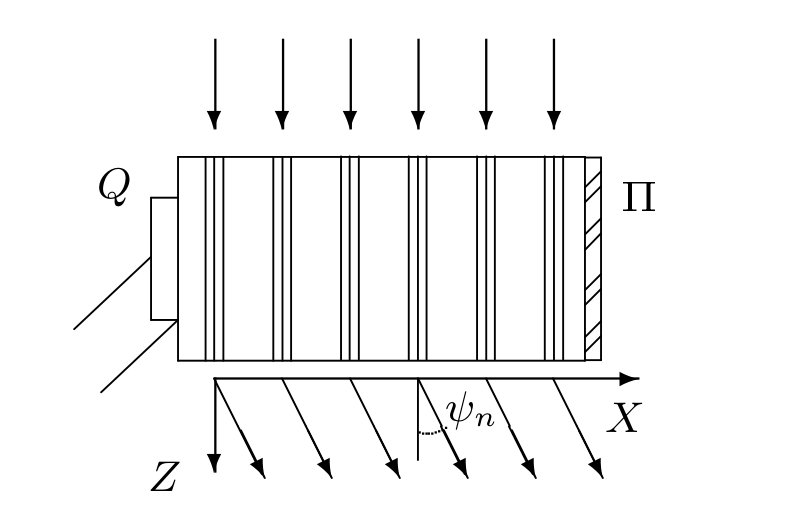
\includegraphics[width = 8cm]{1}}
	\caption{Дифракция световых волн на акустической решетке}
	\label{fig:image}
\end{figure}

Пусть УЗ-волна распространяется вдоль оси Х (рис. 1) в жидкости, налитой в стеклянную кювету в направлении оси Z сквозь жидкость проходит световая волна, испытывающая дифракцию на акустической решётке. Поскольку скорость света значительно больше скорости звука, акустическую решётку можно считать неподвижной. Вызванное ультразвуком возмущение показателя преломления жидкости в нашем акустической решетке случае очень мало. При этом естественно сделать предположение (справедливость которого мы потом ис-
следуем теоретически и экспериментально), что лучи света при прохождении кюветы практически не искривляются.

При небольших амплитудах звуковой волны показатель преломления
жидкости $n$ меняется по закону
\begin{equation}
	n = n_0(1 + a\cos(Kx))
\end{equation}

где К — волновое число для УЗ-волны ($K = 2\pi/\Lambda$), $\Lambda$ -- длина УЗ-волны, а -- глубина модуляции показателя преломления, определяемая интенсивностью ультразвуковой волны (а < 1).

Пусть фаза световых колебаний на передней поверхности жидкости равна нулю. Тогда на задней поверхности (т.е. в плоскости $z = 0$) она равна
\begin{equation}
	\varphi = knL = \varphi_0(1 + a\cos(Kx))
\end{equation}

где $L$ -- толщина слоя жидкости в кювете, $k$ -- волновое число для света ($k = 2\pi/\lambda$), $\lambda$ -- длина световой волны, $\varphi = kn_0L$. Таким образом, в плоскости $z$ = 0 фаза световых колебаний является периодической функцией координаты $x$, иными словами -- УЗ-волна в жидкости создаёт фазовую дифракционную решётку.

Фронт прошедшей через кювету световой волны, т.е. поверхность постоянной фазы, определяется очевидной формулой
\begin{equation}
	z = \frac{\varphi}{k}
\end{equation}

Угол $\Theta(x)$ поворота волнового фронта зависит от координаты $x$:
\begin{equation}
	\Theta(x) = \frac{dz}{dx} = \frac{1}{k}\frac{d\varphi}{dx} = -\frac{K}{k}\varphi_0a\sin(Kx) = -Kn_0L\cdot a\sin(Kx)
\end{equation}

Теперь мы можем сформулировать качественный критерий, при выполнении которого можно пренебречь искривлением световых лучей в кювете и, следовательно, считать акустическую решётку чисто фазовой:
\begin{equation}
	|\Theta(x)|_{max}L \ll \Lambda
\end{equation}

Условие (5) означает, что световой луч (совпадающий с нормалью к волновому фронту) при прохождении кюветы смещается на величину, много меньшую Л, даже если бы он везде внутри жидкости был наклонён под максимально возможным углом $|\Theta(x)|_{max}$. Это условие, конечно, является довольно грубым и содержит большой запас. Опуская несущественные числовые множители, его можно записать в виде
\begin{equation}
	a \ll \left(\frac{\Lambda}{L}\right)^2
\end{equation}

Таким образом, чисто фазовая акустическая решётка реализуется лишь на достаточно слабой УЗ-волне. При повышении мощности ультразвука акустическая волна начинает работать как сложная амплитудно фазовая решётка.

\begin{figure}[h!]
	\center{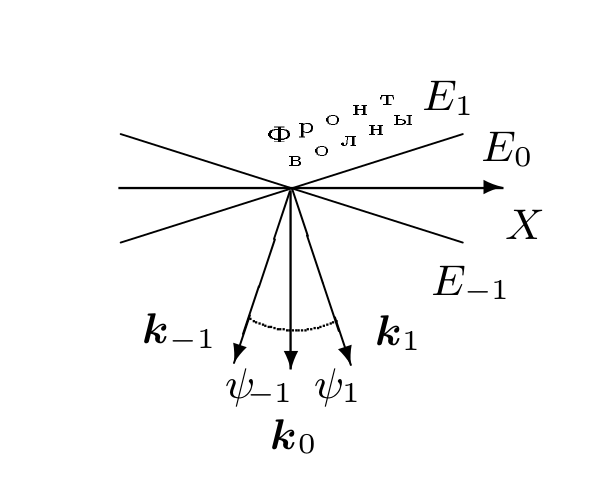
\includegraphics[width = 8cm]{2}}
	\caption{Представление волны в виде суммы трех волн}
	\label{fig:image}
\end{figure}

Дальнейшее рассмотрение будет проведено для случая синусоидальной фазовой решётки методом векторных диаграмм. Световую волну $E$, фаза которой в плоскости $z$ = 0 является гармонической функцией координаты (формула (2)), можно приближённо представить в виде суперпозиции трёх плоских волн $E_0, E_1, E_{-1}$. При этом волна $E_0$ распространяется вдоль оси Z, а направления распространения волн $E_1$ и $E_{-1}$ составляют с этой осью углы $\psi_1$ и $\psi_{-1}$. На рис. 2 изображены волновые векторы
$k_0$, $k_1$, и $K_{-1}$, указывающие направления распространения плоских волн $E_0, E_1, E_{-1}$.

Как следует из рис. 2, фаза волны $E_0$ в плоскости $z$ = 0 не зависит от координаты $x$, а фазы волн $E_1$ и $E_{-1}$ зависят от $x$ по линейному закону. Изобразим теперь колебания $E_0, E_1, E_{-1}$ в некоторой точке $x$ плоскости $z$ = 0 с помощью векторов $E_0, E_1, E_{-1}$ на векторной диаграмме. Тогда при движении $E_0$ вдоль оси X вектор $E_0$ будет оставаться неподвижным, а векторы $Е_1$ и $Е_{-1}$ будут равномерно поворачиваться на векторной диаграмме в разные стороны на углы $\gamma = \pm Kx$. Для того чтобы результирующее колебание $E$, являющееся векторной суммой $E_0, E_1, E_{-1}$, испытывало при этом периодическое изменение фазы и практически не изменялось по амплитуде, взаимная ориентация векторов $E_0, E_1, E_{-1}$ должна соответствовать рис. За при условии, что $E_1$ и $E_2 \ll E_0$.

\begin{figure}[h!]
	\center{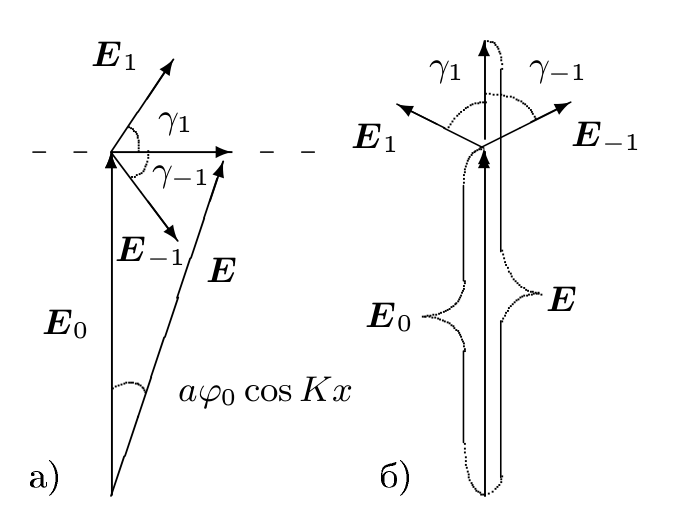
\includegraphics[width = 8cm]{3}}
	\caption{Векторная диаграмма световых колебаний в случае фазовой (а) и амплитудной (б) дифракционной решетки}
	\label{fig:image}
\end{figure}

Чтобы при смешении вдоль оси Х на расстояние, равное длине звуковой волны $\Lambda$, фаза результирующего колебания $E$ возвращалась к прежнему значению, векторы $E_1$ и $E_{-1}$ должны при этом поворачиваться на угол $\pm 2\pi$. Отсюда следует, что углы $\varphi_1$ и $\varphi_{-1}$ должны быть связаны соотношением
\begin{equation}
	\varphi_1 = \varphi_{-1} = \frac{\lambda}{\Lambda}
\end{equation}

где $\lambda$ -- длина световой волны плитудной (6) дифракционной решётки в воздухе. Геометрический смысл соотношения (7) поясняет рис. 4 (на примере волны $E_1$).


Таким образом, при определённых фазовых соотношениях, соответствующих рис. 3, совокупность трёх волн $E_0, E_1, E_{-1}$ правильно описывает в плоскости $z$ = 0 световое поле, фаза которого является гармонической функцией (2) координаты $x$. В силу единственности эта совокупность должна правильно описывать световое поле во всём пространстве за кюветой (т.е. при $z$ > 0). Описанная здесь процедура, называемая разложением светового поля по плоским волнам (метод Релея), широко используется в волновой физике.

\begin{figure}[h!]
	\center{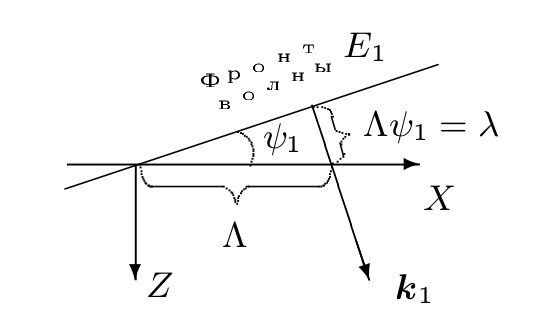
\includegraphics[width = 8cm]{4}}
	\caption{Построение для волны $E_1$}
	\label{fig:image}
\end{figure}

Полезно провести сравнение фазовой и амплитудной акустических синусоидальных дифракционных решёток: для амплитудной решётки фаза световых колебаний при любом значении координаты $x$ постоянна, а амплитуда меняется по гармоническому закону, аналогичному (2). Результирующее колебание $E$ снова может быть представлено в виде суммы трёх
колебаний $E_0, E_1, E_{-1}$ (рис. 3б), однако теперь на векторной диаграмме сумма $E_1 + E_{-1}$ параллельна вектору $E_0$, а не перпендикулярна ему, как это было в предыдущем случае. Таким образом, переход от фазовой решётки к амплитудной соответствует повороту вектора $E_0$ на векторной диаграмме на угол $\pi/2$.

При наблюдении дифракционной картины Фраунгофера три плоские волны $E_0, E_1, E_{-1}$ соответствуют дифракционным максимумам нулевого и первого порядков.

Проведённое выше рассмотрение справедливо только в случае слабой фазовой модуляции. В общем случае после прохождения через кювету световое поле представляет совокупность не трёх, а большого числа плоских волн, распространяющихся под углами, определяемыми условием
\begin{equation}
	\Lambda\sin(\psi_m) = m\lambda,~~(m = 0, \pm1, \pm2, ...)
\end{equation}

Каждая из этих волн соответствует одному из максимумов в дифракционной картине Фраунгофера.

Определяя на опыте положение дифракционных максимумов различного порядка, можно по формуле (8) найти длину $\Lambda$ УЗ-волны и вычислить скорость $v$ распространения ультразвуковых волн в жидкости, если известна частота и колебаний кварцевого излучателя:
\begin{equation}
	v = \Lambda\nu
\end{equation}

Изложенная теория применима как для бегущих, так и для стоячих ультразвуковых волн. Стоячие УЗ-волны образуются при наложении волны, идущей от излучателя, и волны, отражённой от задней стенки кюветы. Если же заднюю стенку кюветы покрыть слоем пористой резины (слой П на рис. 1), то волна от неё не отражается, и в кювете образуется практически чистая бегущая волна. Следует иметь в виду, что в стоячей волне амплитуда изменения давления (а следовательно, и коэффициента преломления) больше, чем в бегущей волне, создаваемой тем же излучателем. В связи с этим дифракционная картина в первом случае содержит большее число максимумов.


\textbf{Экспериментальная установка.} Для наблюдения дифракции света, на УЗ-волнах на оптической скамье собирается установка, изображённая на рис. 5.

\begin{figure}[h!]
	\center{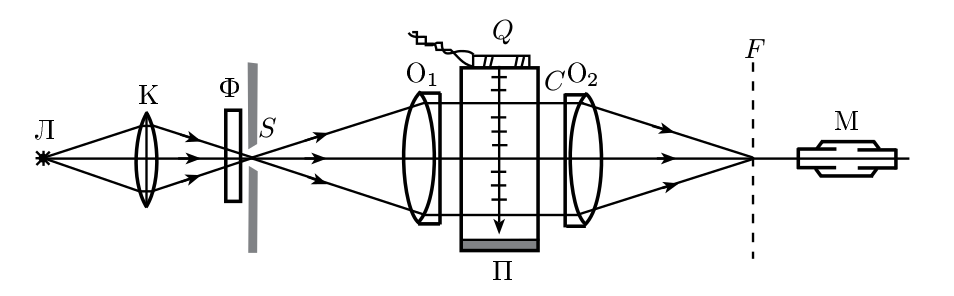
\includegraphics[width = 15cm]{5}}
	\caption{Экспериментальная установка}
	\label{fig:image}
\end{figure}

Источник света Л через светофильтр Ф и конденсор $K$ освещает щель $S$, которая расположена в фокусе объектива $O_1$. Выходящий из объектива параллельный пучок света проходит через кювету С перпендикулярно направлению распространения УЗ-волн. Эти волны возбуждаются в жидкости пьезокварцевой пластинкой $Q$, прикреплённой к стенке кюветы. На кварцевую пластинку подаётся напряжение ультразвуковой частоты от генератора (на рис. 5 не показан). В фокальной плоскости второго объектива $O_2$ образуется дифракционная картина, наблюдаемая при помощи микроскопа $M$. При этом обязательно применяют монохроматическое излучение (красный светофильтр).

Чёткость дифракционных полос зависит от ряда факторов, например, от ширины щели $S$, от её наклона по отношению к вертикали, от угла наклона кюветы к падающему лучу и т.д.

Длина $\Lambda$ ультразвуковой волны определяется с помощью (8); в силу малости углов $\varphi_m$ окончательное выражение может быть представлено в виде
\begin{equation}
	l_m = mf\frac{\lambda}{\Lambda}
\end{equation}

где $l_m$ -- измеренное на опыте линейное расстояние между $m$-м и нулевым максимумами, а $f$ -- фокусное расстояние объектива $O_2$.

\textbf{Наблюдение оптических неоднородностей, создаваемых ультразвуковыми волнами в жидкости методом тёмного поля.} Попробуем теперь получить видимое изображение фазовой акустической решётки. Для этого прежде всего необходимо получить в поле зрения микроскопа изображение задней плоскости (считая по ходу световых лучей) кюветы. Это достигается с помощью вспомогательной положительной линзы О, которую располагают на оптической скамье за фокальной плоскостью объектива $O_2$ (рис. 6).

\begin{figure}[h!]
	\center{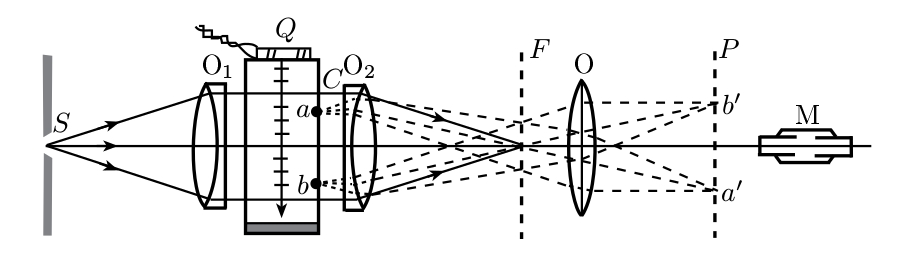
\includegraphics[width = 15cm]{6}}
	\caption{Наблюдение акустической решетки методом темного поля}
	\label{fig:image}
\end{figure}

Перемещая микроскоп вдоль оптической скамьи, фокусируют его на плоскость $P$, где расположено чёткое изображение $a'b'$ какого-либо предмета аб, вплотную прижатого к стенке кюветы. Можно ли теперь увидеть в микроскоп УЗ-волну?

В силу таутохронизма линзы $O_2$ и $O$ изображают кювету в плоскости $P$, не нарушая фазовых соотношений между колебаниями, изображаемыми на диаграмме векторами $E_0, E_1, E_{-1}$ (и векторами высших порядков, если они есть в картине). Диаграмма рис. 3 применима поэтому и к плоскости Р. Освещённость отдельных точек этой плоскости, пропорциональная квадрату амплитуды результирующего светового колебания $E$, в первом приближении не зависит от координаты $x$. Акустическая решётка оказывается, следовательно, невидимой, если, конечно, выполнено условие (6), при котором решётка является чисто фазовой.

Сравнение векторных диаграмм фазовой и амплитудной решёток (см. рис. 3) показывает, что при изменении фазы колебаний в центральном дифракционном максимуме на $\pm\pi/2$ фазовую структуру можно сделать видимой. Такой метод наблюдения носит название метода фазового контраста.

В настоящей работе используется другой способ получения видимого изображения решётки -- метод тёмного поля, основанный на устранении центрального дифракционного максимума с помощью специального экрана. Результирующее колебание на векторной диаграмме представляется при этом суммой только двух векторов $E_1$ и $E_{-1}$. Как следует из рис. За, амплитуда результирующего колебания при этом максимальна при углах поворота векторов $\gamma_1 = \gamma_{-1} = 0,\pi$ и равна нулю при углах $\gamma_1 = \gamma_{-1} = \pi/2, 3\pi/2$. В поле зрения микроскопа наблюдаются чередующиеся светлые и тёмные полосы, причём расстояние между тёмными полосами соответствует смещению в плоскости кюветы на $\Lambda/2$. Таким образом, наблюдается характерное для метода тёмного поля удвоение числа деталей рассматриваемой структуры.

Этот опыт можно проводить только со стоячими волнами, т.к. в случае бегущей волны визуальное наблюдение оказывается невозможным: глаз не успевает следить за быстро перемещающейся волной.

\textbf{Установка с горизонтальной щелью.}

\begin{figure}[h!]
	\center{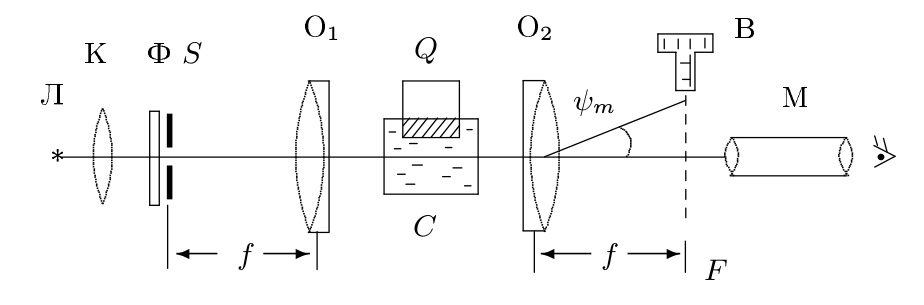
\includegraphics[width = 15cm]{7}}
	\caption{Схема для налюдения дифракции на акустической решетке}
	\label{fig:image}
\end{figure}

Источник света Л (рис. 7) с помощью конденсора К проецируется на входную (коллиматорную) щель 5. Входная щель ориентирована горизонтально и прикрыта красным светофильтром Ф. Коллиматорный объектив $O_1$ посылает параллельный пучок на кювету с водой $C$.

Излучатель $Q$, погружённый в кювету, создаёт УЗ-волну. Вертикальное перемещение излучателя осуществляется винтом $I$ (рис. 8), тонкая подача -- лимбом П. При определённых положениях излучателя волна становится стоячей.

Параллельный пучок света, дифрагируя на стоячей звуковой волне, образует дифракционную картину в фокальной плоскости Р (рис. 7) камерного объектива $O_2$. Картину можно наблюдать в микроскоп М.

Дифракционные полосы ориентированы горизонтально. Расстояние между ними можно измерить с помощью микрометрического винта В. Винт передвигает размещённые на стекле (рис. 9) в плоскости $F$ перекрестие П, тонкую реперную линию $P_{\text{л}}$ и толстую проволоку $\text{П}_p$, которая используется в методе тёмного поля.

Соберем установку, отцентруем источник света и коллиматор. Установим рабочую ширину щели примерно 30 мкм.

Снимем зависимость координаты максимума от номера:

\begin{center}
\begin{tabular}{|c|c|c|c|c|c|c|c|c|c|}
\hline
\multicolumn{2}{|c|}{$\nu = 1.129$ МГц}	&	\multicolumn{2}{|c|}{$\nu = 1.220$ МГц}	&	\multicolumn{2}{|c|}{$\nu = 1.303$ МГц}	&	
\multicolumn{2}{|c|}{$\nu = 1.757$ МГц}	\\
\hline
m	&	$y$	&	m	&	$y$	&	m	&	$y$	&	m	&	$y$	\\
\hline
-2	&	26	&	-2	&	20	&	-2	&	15	&	-2	&	-8	\\
\hline
-1	&	60	&	-1	&	56	&	-1	&	55	&	-1	&	41	\\
\hline
0	&	-6	&	0	&	-4	&	0	&	-5	&	0	&	-6	\\
\hline
1	&	31	&	1	&	34	&	1	&	35	&	1	&	47	\\
\hline
2	&	65	&	2	&	67	&	2	&	74	&	2	&	102	\\
\hline
3	&	99	&	3	&		&	3	&		&	3	&		\\
\hline
\end{tabular}
\end{center}

При этом погрешность измерения $m$ равна нулю, так как номер максимума мы знаем точно, а погрешность $y$ примем равной 1 дел.
Пересчитаем $Y$ - смещение от нуля. Для положительных максимумов это $Y(m) = y(m) - y(0)$, для отрицательных - $Y(m) = -100 - y(0) + y(m)$. При этом погрешность $Y$ будет равна 2дел:

\begin{center}
\begin{tabular}{|c|c|c|c|c|c|c|c|c|c|c|c|}
\hline
\multicolumn{2}{|c|}{$\nu = 1.129$ МГц}	&	\multicolumn{2}{|c|}{$\nu = 1.220$ МГц}	&	\multicolumn{2}{|c|}{$\nu = 1.303$ МГц}	&
\multicolumn{2}{|c|}{$\nu = 1.757$ МГц}	\\
\hline
m	&	$Y$	&	m	&	$Y$	&	m	&	$Y$	&	m	&	$Y$		\\
\hline
-2	&	-68	&	-2	&	-76	&	-2	&	-80	&	-2	&	-102	\\
\hline
-1	&	-34	&	-1	&	-40	&	-1	&	-40	&	-1	&	-53		\\
\hline
0	&	0	&	0	&	0	&	0	&	0	&	0	&	0		\\
\hline
1	&	37	&	1	&	38	&	1	&	40	&	1	&	53		\\
\hline
2	&	71	&	2	&	71	&	2	&	79	&	2	&	108		\\
\hline
3	&	105	&	3	&		&	3	&		&	3	&			\\
\hline
\end{tabular}
\end{center}

Построим график зависимости $Y(m)$:

\begin{tikzpicture}
\begin{axis}[
	height = 10cm,
	width  = 15cm,
	every axis y label/.style={at = {(ticklabel cs: 0.5)}, rotate = 90, anchor = near ticklabel},
	xlabel = {$m$},
	ylabel = {$Y$, дел},
	grid   = major,
]

\addplot+[
	only marks,
	error bars/.cd, 
	y dir = both, y explicit,
	x dir = both, x explicit,
	]
coordinates{
	(-2, -68)
	(-1, -34)
	(0,  0)
	(1, 37)
	(2, 71)
	(3, 105)
};
\addplot [mark = none]
coordinates{
	(-2, -68.4286)
	(3, 105.429)
};

% 34.77

\addplot+[
	only marks,
	error bars/.cd, 
	y dir = both, y explicit,
	x dir = both, x explicit,
	]
coordinates{
	(-2, -76)
	(-1, -40)
	(0,  0)
	(1, 38)
	(2, 71)
};
\addplot [mark = none]
coordinates{
	(-2, -75.8)
	(2, 73)
};
% 37.2

\addplot+[
	only marks,
	error bars/.cd, 
	y dir = both, y explicit,
	x dir = both, x explicit,
	]
coordinates{
	(-2, -80)
	(-1, -40)
	(0,  0)
	(1, 40)
	(2, 79)
};
\addplot [mark = none]
coordinates{
	(-2, -79.8)
	(2, 79.4)
};
% 39.8

\addplot+[
	only marks,
	error bars/.cd, 
	y dir = both, y explicit,
	x dir = both, x explicit,
	]
coordinates{
	(-2, -102)
	(-1, -53)
	(0,  0)
	(1, 53)
	(2, 108)
};
\addplot [mark = none]
coordinates{
	(-2, -104)
	(2, 106.4)
};
% 52.6

\end{axis}
\end{tikzpicture}


Из формулы (10) следует:
$$
	l_m = mf\frac{\lambda}{\Lambda} \Rightarrow \Lambda = \frac{m}{l_m}\lambda f
$$
То есть, зная угловой коэффициент графиков, можно найти $\Lambda$.

По МНК определим значение $k$ и его случайную погрешность. Полную погрешность найдем по формуле
$$
	\sigma = \sqrt{\sigma_\text{случ}^2 + \sigma_\text{приб}^2}
$$

\begin{center}
\begin{tabular}{|c|c|c|c|c|c|c|c|c|c|c|}
\hline
$\nu$, МГц					&	1.129	&	1.220	&	1.303	&	1.757	\\
\hline
$k$, дел					&	35		&	37		&	40		&	53		\\
\hline
$\sigma_\text{случ}$, дел	&	1		&	1		&	1		&	1		\\
\hline
$\sigma$, дел				&	2		&	2		&	2		&	2		\\
\hline
\end{tabular}
\end{center}

Откуда, зная, что $f = 28$см и $\lambda = (640 \pm 20)$нм:
$$
	1.129 \text{МГц}:~~(130 \pm 10)\cdot10^{-5}\text{м};~~(1470\pm130)\text{м/с}
$$
$$
	1.220 \text{МГц}:~~(120 \pm 10)\cdot10^{-5}\text{м}:~~(1460\pm130)\text{м/с}
$$
$$
	1.303 \text{МГц}:~~(110 \pm 10)\cdot10^{-5}\text{м}:~~(1430\pm140)\text{м/с}
$$
$$
	1.757 \text{МГц}:~~  (85 \pm 8)\cdot10^{-5}\text{м}:~~(1490\pm150)\text{м/с}
$$

\vspace{1cm}
Для метода темного поля определим цену деления шкалы окуляра: 1мм = 25дел. Отсюда: $1 \text{дел} = 40\cdot10^{-6}\text{м}$.

Снимем зависимость первой и последней хорошо видимых темных полос и число светлых промежутков между ними от частоты:

\begin{center}
\begin{tabular}{|c|c|c|c|c|c|c|c|c|c|c|}
\hline
$\nu$, МГц	&	x, дел	&	y, дел	&	N	&	$\Lambda$, мм	&	$\sigma_\Lambda$, мм	&	$1/\nu$, МГц$^{-1}$	\\
\hline
1.258		&	5		&	135		&	9	&	1.15			&	0.02					&	0.795				\\
\hline
1.347		&	10		&	130		&	9	&	1.07			&	0.02					&	0.742				\\
\hline
1.434		&	2		&	128		&	10	&	1.01			&	0.02					&	0.697				\\
\hline
1.583		&	2		&	128		&	11	&	0.92			&	0.02					&	0.632				\\
\hline
1.521		&	8		&	125		&	10	&	0.94			&	0.02					&	0.657				\\
\hline
1.693		&	4		&	126		&	11	&	0.89			&	0.02					&	0.591				\\
\hline
1.954		&	0		&	122		&	13	&	0.75			&	0.02					&	0.512				\\
\hline
1.810		&	0		&	120		&	12	&	0.81			&	0.02					&	0.552				\\
\hline
1.200		&	10		&	128		&	8	&	1.18			&	0.02					&	0.833				\\
\hline
\end{tabular}
\end{center}

$\Lambda$ найдем по формуле
$$
	\Lambda = \frac{y-x}{N}h,
$$
\noindent где $h$ - цена деления окуляра.

Принимая погрешность х и у равной 1дел, нетрудно найти погрешность $\Lambda$.

Теперь построим график $\Lambda(1/\nu)$:


\begin{tikzpicture}
\begin{axis}[
	height = 10cm,
	width  = 15cm,
	every axis y label/.style={at = {(ticklabel cs: 0.5)}, rotate = 90, anchor = near ticklabel},
	xlabel = {$1/\nu$, МГц$^{-1}$},
	ylabel = {$\Lambda$, мм},
	grid   = major,
]
\addplot+[
	only marks,
	error bars/.cd, 
	y dir = both, y explicit,
	x dir = both, x explicit,
	]
coordinates{
	(0.795, 1.15) +- (0, 0.02)
	(0.742, 1.07) +- (0, 0.02)
	(0.697, 1.01) +- (0, 0.02)
	(0.632, 0.92) +- (0, 0.02)
	(0.657, 0.94) +- (0, 0.02)
	(0.591, 0.89) +- (0, 0.02)
	(0.512, 0.75) +- (0, 0.02)
	(0.552, 0.81) +- (0, 0.02)
	(0.833, 1.18) +- (0, 0.02)
};
\addplot [mark = none]
coordinates{
	(0.512, 0.759677)
	(0.833, 1.19048)
};

\end{axis}
\end{tikzpicture}

Из графика по МНК определим $v = \frac{d\Lambda}{d(1/\nu)}$. Случайную погрешность определим также по МНК, приборную же найдем, считая $v = f(\Lambda, 1/\nu)$. Таким образом:
$$
	v = (1.36 \pm 0.08)\cdot10^3\text{м/с}
$$

\newpage
Таким образом, в данной лабораторной работе мы изучили дифракцию света на акустической решетке и определили скорость волн, используя метод темного поля.










\end{document}